\documentclass[longbibliography,nofootinbib,twocolumn]{revtex4-1}

\newcommand{\nucypher}{NuCypher}

\usepackage{listings}
\usepackage{graphicx}
\usepackage{amsmath}
\usepackage[margin=5pt]{subfig}
\usepackage[usenames]{color}

\renewcommand{\baselinestretch}{1.4}
\setlength{\parskip}{1em}
\definecolor{darkgreen}{rgb}{0.00,0.50,0.25}
\definecolor{darkblue}{rgb}{0.00,0.00,0.67}
\newcommand{\figref}[1]{Fig.~\ref{#1}}
\usepackage[breaklinks,pdftitle={NuCypher: Mining \& Staking Economics}, pdfauthor={Michael Egorov, MacLane Wilkison},colorlinks,urlcolor=blue,citecolor=darkgreen,linkcolor=darkblue]{hyperref}
\graphicspath{{pdf/}}

\usepackage[T1]{fontenc}
\usepackage{lmodern}
\lstset{
    basicstyle=\ttfamily,
    basewidth={0.5em, 0.5em},
    columns=fullflexible,
}

\begin{document}

\title{\nucypher: Mining \& Staking Economics}

\author{Michael Egorov, MacLane Wilkison}
\email{michael@nucypher.com, maclane@nucypher.com}
\affiliation{NuCypher}

\begin{abstract}
This paper describes mining mechanisms and economics in the \nucypher~network.
The paper covers inflation rates, mechanisms to incentivize staking over the long-term,
and estimates of the number of tokens that will be earned by nodes running in typical modes.
Finally, a number of price volatility mitigation strategies are proposed.
\end{abstract}

\date{\today}
\maketitle

\section{Motivation}

Upon deployment of the \nucypher~network, and as the number of developers and applications using \nucypher~grows, payment for re-encryption services (`network fees') will account for an increasing proportion of earnings made by network nodes.
However, before developer adoption has reached a sufficient threshold, nodes must be incentivized via a block compensation subsidy.
This can be achieved via an inflation schedule that is distributed exclusively to miners.

An ideal compensation model should have the following properties:
\begin{itemize}
    \item The inflation distributed to stakers is proportional to their stake;
    \item The amount of work assigned to stakers (and, hence, compensation earned) is proportional to their stake;
    \item Stakers are incentivized (by a higher compensation rate) to run nodes for longer periods;
    \item Periods of high inflation do not significantly depreciate the token price, maintaining liquidity for new stakers;
    \item Stakers are strongly incentivized to stay online all the time, in order to maximize availability to users requiring re-encryption services;
    \item Stakers are incentivized to `re-stake' inflation compensation in order to maximize their long-term compensation;
    \item Short-term staking is also encouraged and subsidized, albeit at a lower rate.
\end{itemize}

This paper addresses each of these desired properties, calculates expected miner compensation, and devises optimal mining/staking strategies.

\section{Historical examples of inflation}

Let's review inflation schedules of different cryptocurrency projects:
DASH~\cite{dash:whitepaper} and ZCash~\cite{zcash}.

DASH has a hybrid Proof-of-Work (POW) and Proof-of-Stake (POS) model,
with $45\%$ of inflation going to POW miners, $45\%$ to staking master nodes, and $10\%$ reserved for budget proposals~\cite{dash:emission}.
After the first year, its emission was $18.42\%$ APR, decreasing by $1/14$ every $383$ days.
With this setting, $60\%$ of DASH coins are locked in masternodes for staking.
It's unclear how inflation rate affects the price (and if it does here), but the useful data point is that there are $60\%$ of coins locked for staking.
Perhaps, that is a reasonable starting point to expect in a network where staking is an option.

% TODO: replot in a more reasonable shape
\begin{figure}
    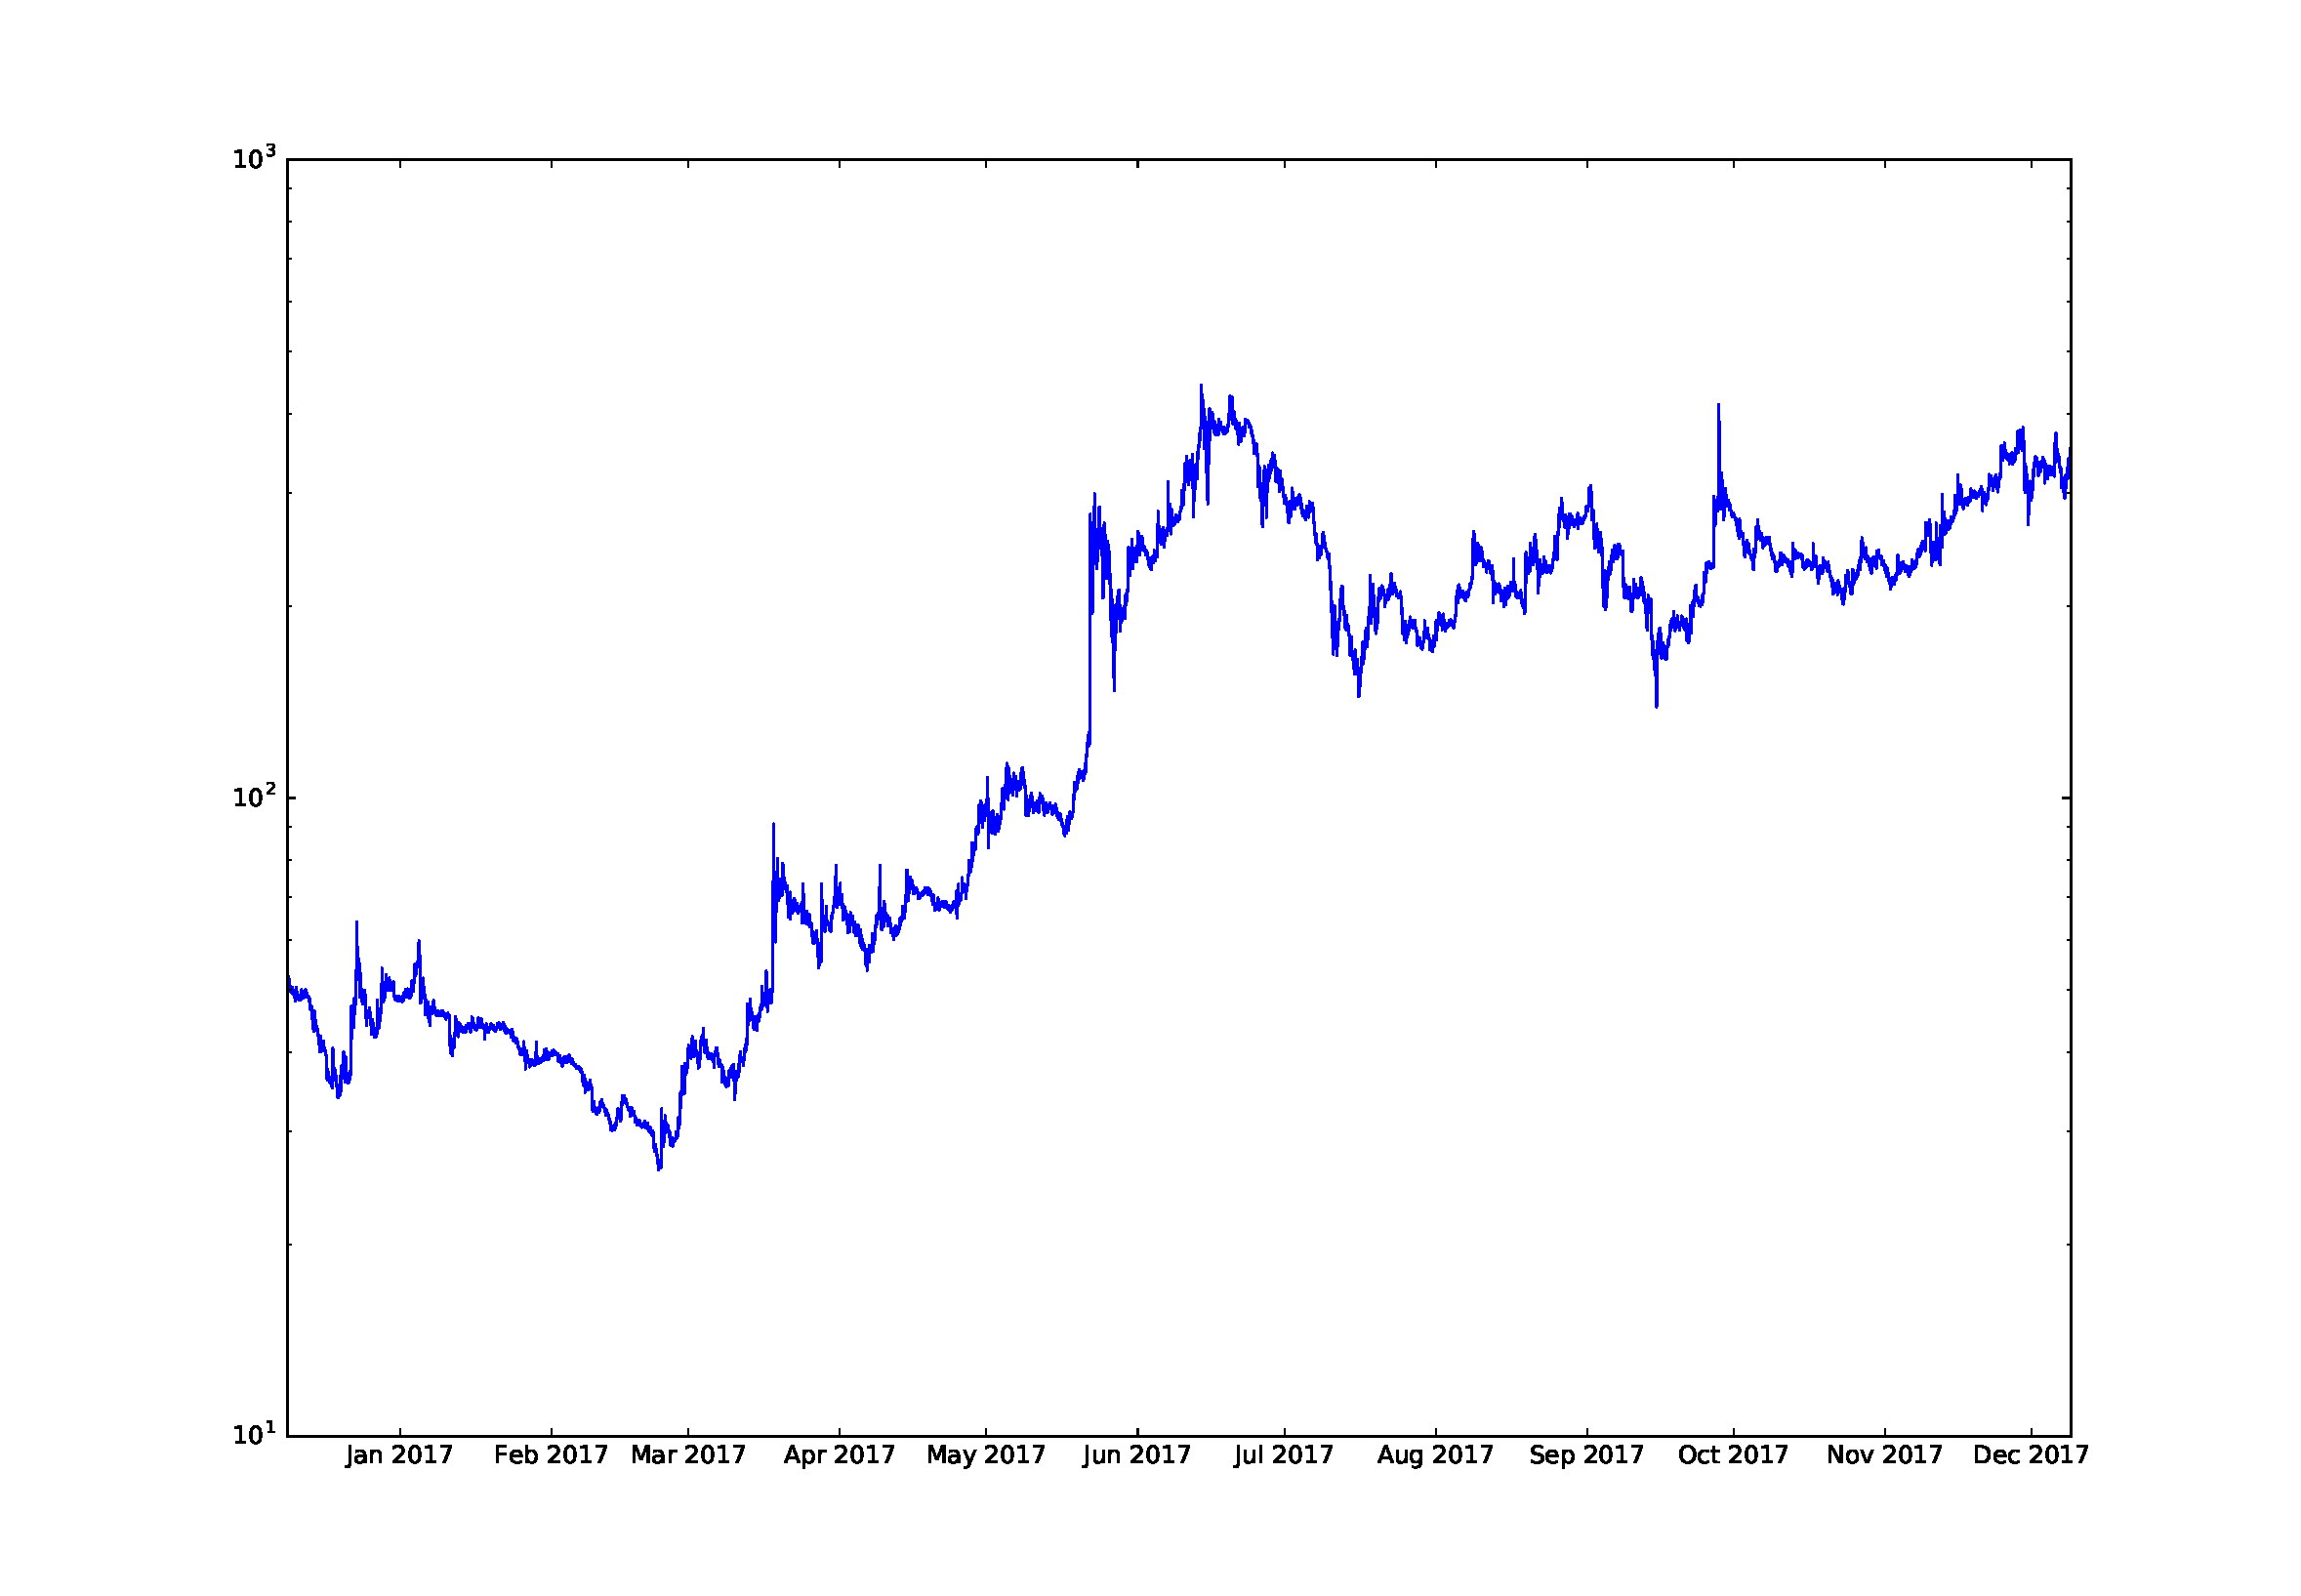
\includegraphics[width=\columnwidth]{pdf/zcash-price.pdf}
    \caption{Historical price of ZCash in logarithmic scale. Note the minimum at 23 Feb 2017}
    \label{fig:zec}
\end{figure}

ZCash is very interesting because it started with an extremely high inflation rate.
This caused a short-term price drop (even though the market capitalization was growing)~(\figref{fig:zec}).
But on 23~Feb~2017, the price started going up.
ZCash block rewards yield $50$~ZEC every $10$~min, and ZEC supply at Feb~23 was $727$k~ZEC.
This corresponds to $360\%$~APR.
It is even more remarkable given the fact that miners who mined ZEC are likely selling and exchanging the proceeds into other currencies to cover expenses.
This gives us information about the maximum allowable inflation which doesn't create too much downward pressure on the price.

\section{Mining protocol}

A miner commits to stay available for at least time $T$.
For that, they specify an unlocking time $t_1$,
where minimal lock time $t_1 - t$ should be not less than $T_{\min} = 1$~month.
The number of coins locked for staking $l$ should be no less than $S_{\min}$.

\begin{figure}
    \subfloat[Unlocking in a single step]{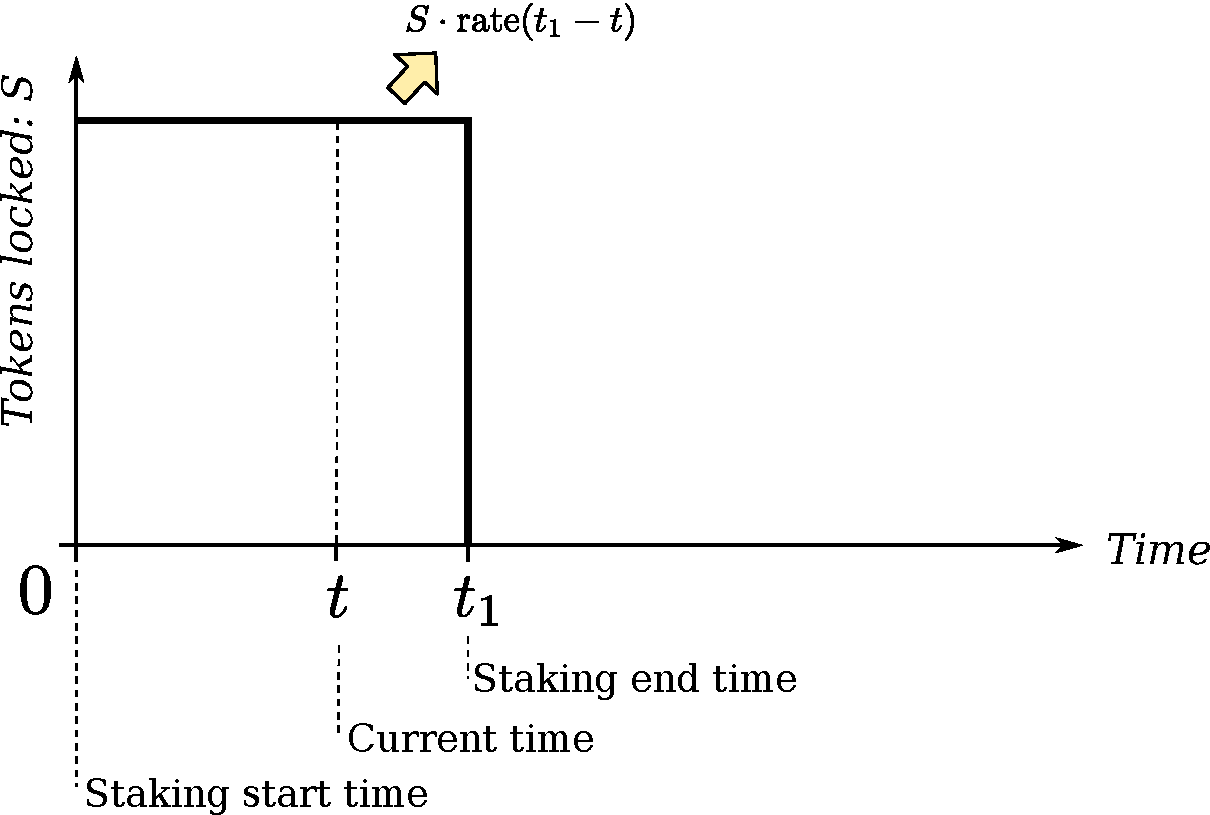
\includegraphics[width=\columnwidth]{pdf/one-step.pdf}}\\
    \subfloat[Splitting into two steps]{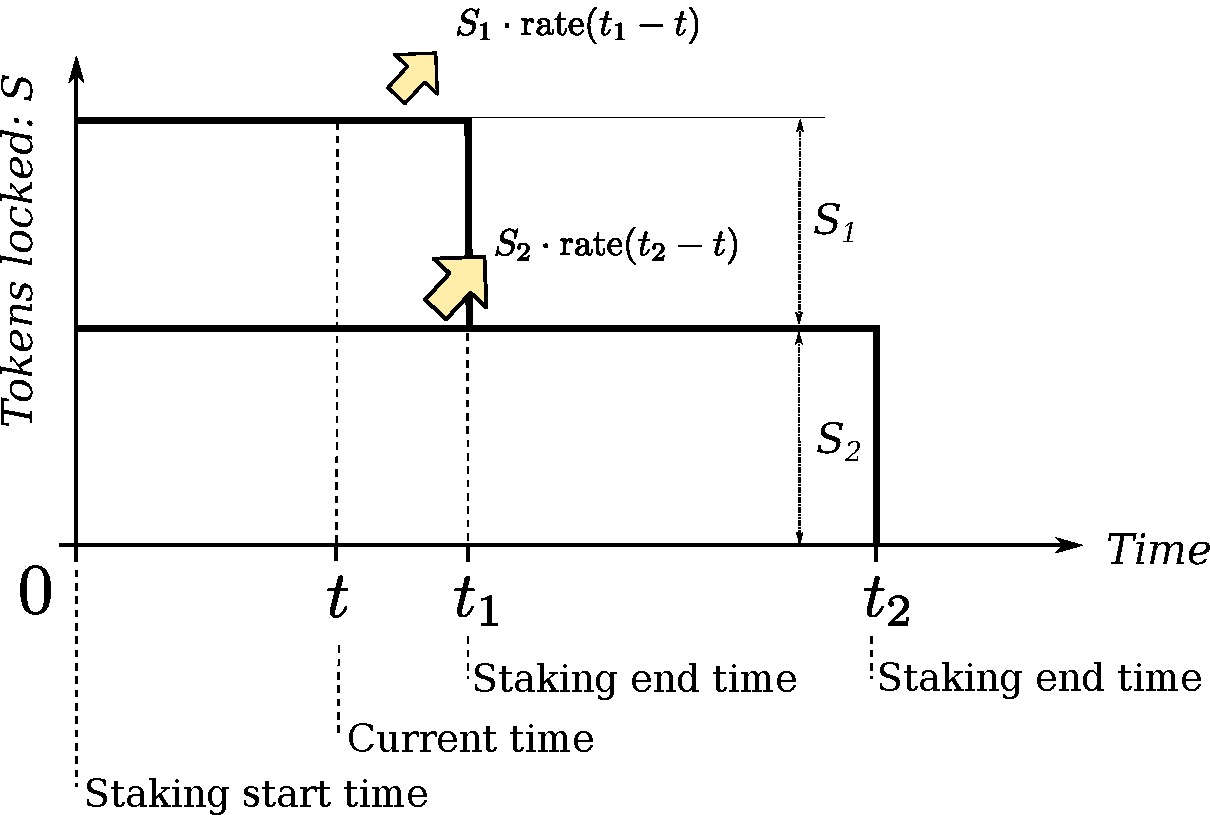
\includegraphics[width=\columnwidth]{pdf/two-steps.pdf}}
    \caption{
        When staked, an unlock time $t_1$ is specified.
        At any time the unlock time can be increased (but not decreased).
        The stake can optionally be split into two parts where only one part is extended to $t_2$.
    }
    \label{fig:mining-modes}
\end{figure}

At any point, a miner can split their stake or any piece of their stake into two pieces~(\figref{fig:mining-modes}).
The size of each piece should be not less than $S_{\min}$.
The reason miners may want to split their stake is because their compensation rate depends on the lock time $T$,
which will be discussed in more details later.
At any point the miner can increase (but not decrease) $T$ and add more tokens to their stake.

\section{General inflation properties}

\subsection{Initial inflation}

Let's assume that \nucypher~will have the same number of tokens locked as DASH: $\lambda=60\%$.
Thus, we'll have $1-\lambda=40\%$ in circulation.
If the inflation rate is $I$, then the adjusted inflation rate (i.e. inflation as if the locked tokens didn't exist) of tokens in circulation will be:
\begin{equation}
    I^* = \frac{I}{1-\lambda},
\end{equation}
and we should be comparing $I^*$ with historical examples of inflation.
If we take $I^*=350\%$ (turnover point of ZCash price in an overall bullish market), the corresponding inflation $I$ will be $140\%$~APR.

To err on the side of caution, we set the starting inflation to be $I_0=100\%$~APR (or, in other words, $1/365$ per day).

\subsection{Inflation decay}

Initially, inflation subsidizes mining, but payments for re-encryption services will generate the majority or all of the revenues of miners in the long run.
If all miners have the same, maximum compensation rate, we choose the inflation rate to decay by factor of $2$ in $T_{1/2} = 2$ years.
The inflation, depending on time passed from the Genesis $t$, looks like:
\begin{equation}
    I(t) = I_0 \cdot 2^{-\frac{t}{T_{1/2}}} = I_0 \exp\left[ -\ln{2} \frac{t}{T_{1/2}} \right].
\end{equation}
In this case, the dependence of the token supply on the time $t$ is:
\begin{equation}
    \label{eq:supply-time}
    S(t) = S_0 + \int_0^{t} I(t)\, dt = S_0 + \frac{I_0 T_{1/2}}{\ln{2}}\left[1 - 2^{-\frac{t}{T_{1/2}}} \right],
\end{equation}
Let's call relative initial annual inflation $i_0$, and then $I_0 = i_0 S_0$.
For $100\%$~APR, $i_0=1$ and $I_0=S_0$~per~year, and the maximum number of tokens which will ever be created is:
\begin{equation}
    S_{\max} = S(\infty) = S_0\left(1 + \frac{i_0 T_{1/2}}{\ln{2}}\right) \approx 3.89\, S_0,
\end{equation}
where $S_0$ is initial number of tokens.

\subsection{Implementation of the exponential decay in a smart contract}

Complex functions like exponentials, if implemented in smart contracts, would be quite costly.
Fortunately, the exponential is a solution of a differential equation where inflation is proportional to the amount of not yet mined tokens:
\begin{eqnarray}
    I(t) &=& \frac{\ln{2}}{T_{1/2}} \left( S_{\max} - S(t) \right)\\
    dS &=& I(t)\, dt,
\end{eqnarray}
where $S(t)$ is the current token supply with $S(0)=S_0$ and the time step $dt$ can actually be equal to the mining period ($1$~day).
Each mining node can trivially calculate its $dS$ in a smart contract using very few operations and the coin supply $S$ from the last period.
So, the amount of tokens mined for the node $i$ and the time period $t$ will be:
\begin{eqnarray}
    \label{eq:rate-max}
    ds_{i,t} &=& \frac{l_i}{L} \frac{\ln{2}}{T_{1/2}} \left( S_{\max} - S_{t-1} \right),\\
    dS_t &=& \sum_i ds_{i,t},
\end{eqnarray}
where $l_i$ is the number of tokens locked by the miner $i$, $L$ is the total number of tokens locked.
Instead of calculating all the sum over $i$, each miner $i$ can add her portion $ds_{i,t}$.

\subsection{Mining rate and staking time}

\begin{figure}
    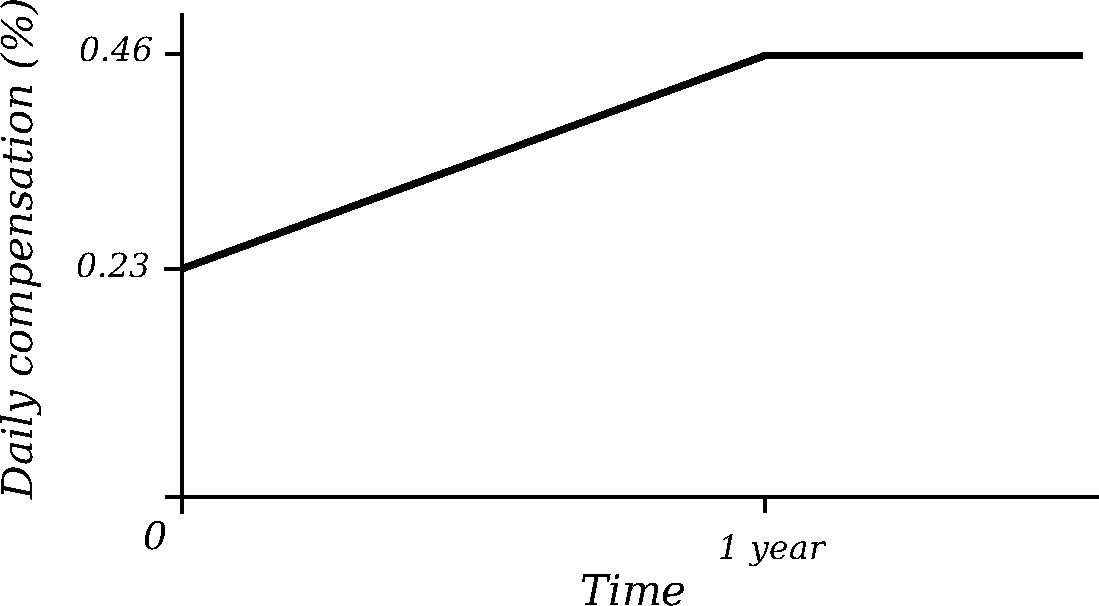
\includegraphics[width=\columnwidth]{pdf/rate.pdf}
    \caption{Dependence of the compensation rate on staking duration. We assume $60\%$ of all tokens locked for staking}
    \label{fig:reward-rate-vs-duration}
\end{figure}

We want to incentivize miners to serve re-encryption policies for at least $1$~year.
However, short-term stakers are still useful and should be compensated.
We will give the full compensation ($\kappa=1$) to the stakers who are committed to stake at least $T_1=1$~year,
however those who stake for $T_{\min}=1$~month will get close to half the compensation ($\kappa\approx0.54$) (\figref{fig:reward-rate-vs-duration}).
The individual daily compensation rate for a miner looks as:
\begin{eqnarray}
    \kappa &=& \left(0.5 + 0.5\frac{\min(T_i, T_1)}{T_1}\right)\\
    T_{i,\text{initial}} &\ge& T_{\min},\\
    \delta s_{i,t} &=&  \kappa\, \frac{l_i}{L} \frac{\ln{2}}{T_{1/2}} \left( S_{\max} - S_{t-1}\right).\\
\end{eqnarray}
The unlocking time $T_i$ means the time left to unlock the tokens $t_1 - t$.
The initial $T_i$ cannot be set smaller than $1$~month,
but it eventually becomes smaller than that as the time passes, and the miner gets close to unlocking the stake.

This has implications on the global token economy.
Firstly, if stakers, despite smaller compensation, prefer to stake for shorter time periods, that results in a smaller daily token emmission.
Since miners will likely prefer shorter stake times during bear markets, reducing the issuance rate during that time will provide better price support and stability
as a side benefit.

Interestingly, $\kappa < 1$ prolongs the compensation half-decay time $T_{1/2}^* = T_{1/2} / \kappa^*$, where $\kappa^*$ is the mean staking parameter.
If all the stakers have $\kappa^* = \kappa = 0.5$, this prolongs $T_{1/2}$ to be $4$~years instead of $2$.

The total supply over time (Eq.~\ref{eq:supply-time}) at $\kappa^* \ne 1$ will then look like:
\begin{equation}
    \label{eq:adjusted-supply-time}
    S(t) = S_0 \left[1 + \frac{i_0 \kappa^* T_{1/2}^*}{\ln{2}}\left(1 - 2^{-\frac{t}{T_{1/2}^*}} \right) \right].
\end{equation}

\section{Mining strategies and expected compensation}

In this section, we look at three possibilities:
a miner liquidating all the compensation while extending the lock time (Stake and Earn),
a miner adding all the compensation to their current stake (Restake),
and a miner waiting for their stake to unlock after time $T$ (Spindown).
Each of these possibilities could have different distributions of $\kappa$.
Let's consider $\kappa=1$ and $\kappa=0.5$ as two marginal values.
Let's take the amount of tokens locked to be $\lambda=60\%$, as in DASH.
We'll plot graphs of daily compensation, as well as calculate the compensation during the first year in each of these scenarios.

\subsection{Stake and Earn: Liquidate mining compensation}

This is the simplest case.
The total amount of tokens staked in the network can be expressed as $L=\lambda S$.
The amount of stake stays constant in this case and equal to $s_i = l$, and the mining rate (i.e. the cumulative compensation) is:
\begin{equation}
    \frac{dr}{dt} =  \kappa\, \frac{l}{\lambda S(t)} \frac{\ln{2}}{T_{1/2}} \left( S_{\max} - S(t)\right).
\end{equation}
Daily compensation $dr/dt$ plotted for $\lambda=0.6$ is shown on \figref{fig:daily-compensation}.

\begin{figure}
    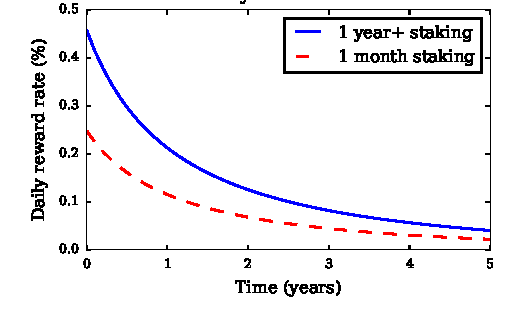
\includegraphics[width=\columnwidth]{pdf/daily-compensation.pdf}
    \caption{Daily compensation over time assuming $60\%$ tokens locked for lock times of $1$~year and $1$~month}
    \label{fig:daily-compensation}
\end{figure}

When we substitute $S(t)$ from Eq.~\ref{eq:adjusted-supply-time} and integrate over time, we find total compensation:
\begin{equation}
    r(t) = l \frac{\kappa}{\kappa^* \lambda} \ln\frac{S(t)}{S_0}.
\end{equation}

If $\kappa=1$ (staking for $1$~year+) and $\lambda=60\%$ ($60\%$ of all nodes in the network are staking),
miner's compensation starts from $0.46\%$~per~day in NU tokens,
or $100.2\%$ during the first year of staking.

We should note that if other miners stake for less than a year ($\kappa^* < 1$), the inflation rate decays slower, and the compensation over a given period
will be higher.

\subsection{Restake mining compensation}

Instead of liquidating mining compensation, it could be restaked into the node in order to increase the miner's stake and, provided the node's hardware is
powerful enough to support the additional workload, earn higher compensation.
In this case, the actual stake $l$ is constantly increasing with time:
\begin{equation}
    \frac{dl}{dt} =  \kappa\, \frac{l}{\lambda S(t)} \frac{\ln{2}}{T_{1/2}} \left( S_{\max} - S(t)\right).
\end{equation}
If we substitute $S(t)$ from Eq.~\ref{eq:adjusted-supply-time} and solve this differential equation against $l$, we get:
\begin{equation}
    l(t) = l(0)\,\left[ \frac{S(t)}{S_0} \right]^{\frac{\kappa}{\kappa^* \lambda}}.
\end{equation}
If $\kappa=1$ (staking for $1$~year+) and $\lambda=60\%$ ($60\%$ of all nodes in the network are staking),
miner's compensation starts from $0.46\%$~per~day in NU tokens,
or $l(1) - l(0) = 177.5\%$ during the first year of staking.
The difference between restaking and taking the compensation is shown at~\figref{fig:total-compensation}.


\begin{figure}
    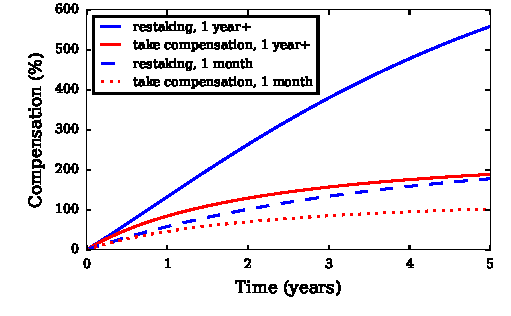
\includegraphics[width=\columnwidth]{pdf/total-compensation.pdf}
    \caption{Total amount of compensation produced by staking with relocking (blue) and without (red),
        when staking for $1$~year or more (solid lines) or $1$~month.}
    \label{fig:total-compensation}
\end{figure}

\subsection{Take mining compensation and spindown}

When the node spins down, the miner doesn't extend the time for end of staking $t_1$,
and the compensation is constantly decreasing as the time left to unlock becomes smaller and smaller,
effectively decreasing $\kappa$ gradually towards $0.5$.
That's the default behavior: to avoid that, the miner should set $t_1$ large enough, or increase $t_1$ periodically.

\subsection{Edge case: connection problems}

If a miner is found to be non-operational and/or cannot confirm its continued performance, the tokens aren't unlocked (and compensation isn't earned).
It's not fatal for the miner if that happens (i.e. their entire stake won't be slashed), however their tokens will remain locked without earning compensation,
until they satisfy their commitment.
So if the miner commits to stake for at least a year, it implies a year of operation.

Connection problems may also be downtime when the miner upgrades their node's software, which is an absolutely legitimate reason to be offline for a short time.

\section{TLDR}

\subsection{How much will I be compensated if I run a node?}
It depends on how early you start (the earlier, the better), and for how long you commit to provide re-encryption services.
If you commit to work for $1$~month, you'll be getting approximately $54\%$ of what you'll be getting if you commit for $1$~year or more.
Also the compensation is inversely proportional to the total amount of tokens staked by all the participants.
Finally, if you choose to automatically restake the tokens, this will increase your total compensation because your stake will be increasing as
well as the amount of work done for the network.

For example, if $60\%$ of tokens in the system are always staked, you'd be earning $0.46\%$ on day $1$.
With this amount of stakers, if you withdraw all the earned tokens instead of restaking them, you'd earn $100.2\%$ of your stake in the first year.
But if you restake all your tokens, in the same first year you'd earn $177.5\%$ of the tokens you staked.

\subsection{How many tokens will ever be in existence?}
We'll start with $1$~billion tokens, and the maximum amount of tokens ever mined will be $3.89$~billion.

\subsection{What's the inflation rate?}
The inflation rate will depend on how many short-term miners and long-term miners are working in the system.
Depending on this, the initial inflation will be between $50\%$~APR (if all miners are very short term) and $100\%$~APR (if all miners commit for a long
term).
The inflation will decay exponentially every day, halving sometime between $2$~years (if all the miners are long term)
and $4$~years (if all the miners are short term).

\bibliography{mining-paper}

\end{document}
